\begin{figure}[ht]
    \centering
    % \begin{forest}
    %     forked edges,
    %     for tree={draw,align=center,edge={-latex}}
    %     [\est{Xorg}
    %         [\est{Xlib}
    %             [\texttt{xrandr}
    %                 [Aplicació]
    %             ]
    %         ]
    %     ]
    % \end{forest}

    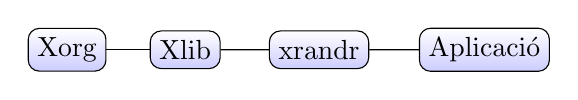
\begin{tikzpicture}[
        grow = right,
        every node/.style = {shape=rectangle, rounded corners,
          draw, align=center,
          top color=white, bottom color=blue!20}]
        \node {\est{Xorg}}
            child {
                node {\est{Xlib}} 
                child {
                    node [xshift=0.2cm] {\est{xrandr}}
                    child {
                        node [xshift=0.6cm] {Aplicació}
                    }
                }
            };
    \end{tikzpicture}

    \caption{Intermediaris entre \est{Xorg} i l'aplicació final \cite{Xrandr}.}
    \label{fig:xorg-hyerarchy}
\end{figure}
